% This is a comment
% https://sites.math.washington.edu//~perkins/300CSpr11/typesetting.php
% This file was downloaded from above and modified 
% Everything from the top of the file to the \begin{document} is
% called the preamble.  It contains information used to set up 
% the document.

\documentclass{article}  
% This has to be the first non comment line of the document.  It tells you what kind
% of document it is.  options: book, article, letter, memo, report, ...

%Below two packages needed for figures
\usepackage{graphicx}
\usepackage{float}




\begin{document}  % This is where the document starts.

\title{A Simple Fucking Example Using \LaTeX}   % \LaTeX makes a fancy LaTeX logo.
\author{R. J. LeVeque and T. P. Chartier}
\date{\today}
\maketitle

\abstract{This short paper illustrates basic techniques in the 
use of the \LaTeX~ text formatting language, which is useful in typesetting  scientific and mathematical papers. This paper can serve as a short tutorial and as a useful template for a beginning \LaTeX~ programmer.}
% ~ denotes a forced space.  Remove the ~ appended to the end of \LaTeX and see what happens.
% Latex is also case sensitive.  If you type \LaTex, you will receive a compiling error.

\section{Introduction}

This paper illustrates how various typesetting is accomplished in \LaTeX. First, notice that components of your paper such as {\it sections, subsections,} and {\it equations} are numbered automatically.  

\subsection{Lists}
Making an itemized list is easy:
\begin{itemize}
\item If the \LaTeX~ file is called {\tt sample.tex} then output is created by executing \\
   {\tt pdflatex sample} \\
\item % and this is a comment that won't print.
To force a line to end, use double backslash as in the previous item as seen in {\tt sample.tex}.

\item Anything after a \% is a comment that won't appear in the output. 
% We are using \tt - to turn on typewriter font.
   % so you need to use the special macro \% if you want % to show up!!
\item This shows the effect of typesetting. Some of the \textbf{greatest} discoveries in \underline{science} were made by \textbf{\textit{accident}}
\end{itemize}

\section{Mathematical formulas}

% This is a citation.  Look at the bibliography to see the reference!
For more information on math formulas, see a \LaTeX~ manual such as \cite{go-mi-sa:latex}.  

This paper supplies only a taste of how mathematical formulas are created in \LaTeX.  As a short introduction, a few pointers are contained in this section. 

Dollar signs places \LaTeX~ into its math mode, which is where mathematical formulas and equations are created.  To include an equation in a current line of text, place one dollar sign (\$) before 
and after the equation, for example we might define $f(x) = 3e^x$.   If an equation should be displayed in another line. See below.
\[ \sum_{j=1}^N j = \frac{N(N+1)}{2}. \]
If the equation should be numbered, use the following notation:
\begin{equation}  
e^{i\pi} = \cos(\pi) = -1.
\label{cosequation}
\end{equation}
This equation was given a label (which is optional).  Hence, the equation can be referred to later as (\ref{cosequation}) rather than hardcoding such numbers into the \LaTeX~ file.  Therefore, adding new equations does not facilitate a need for the programmer to manually renumber the equations. 

(Note that you will have to run \LaTeX~ twice on your {\tt .tex}
file for numbering to appear properly.  The first run stores the labels in the file {\tt sample.aux} and the second time run reads these labels at the beginning of processing.)


More complex math is as under:

Subscripts in math mode are written as $a_b$ and superscripts are written as $a^b$. These can be combined and nested to write expressions such as

\[ T^{i_1 i_2 \dots i_p}_{j_1 j_2 \dots j_q} = T(x^{i_1},\dots,x^{i_p},e_{j_1},\dots,e_{j_q}) \]
 
We write integrals using $\int$ and fractions using $\frac{a}{b}$. Limits are placed on integrals using superscripts and subscripts:

\[ \int_0^1 \frac{dx}{e^x} =  \frac{e-1}{e} \]

Lower case Greek letters are written as $\omega$ $\delta$ etc. while upper case Greek letters are written as $\Omega$ $\Delta$.

Mathematical operators are prefixed with a backslash as $\sin(\beta)$, $\cos(\alpha)$, $\log(x)$ etc.


\section{Figures and Tables}
\subsection{Figures}
To include figures, you can use the includegraphics package as listed below. It supports different extensions (pdf, jog, png etc). 
The first figure has a pdf extension and latter a png.
\begin{figure}[H]
	\centering
	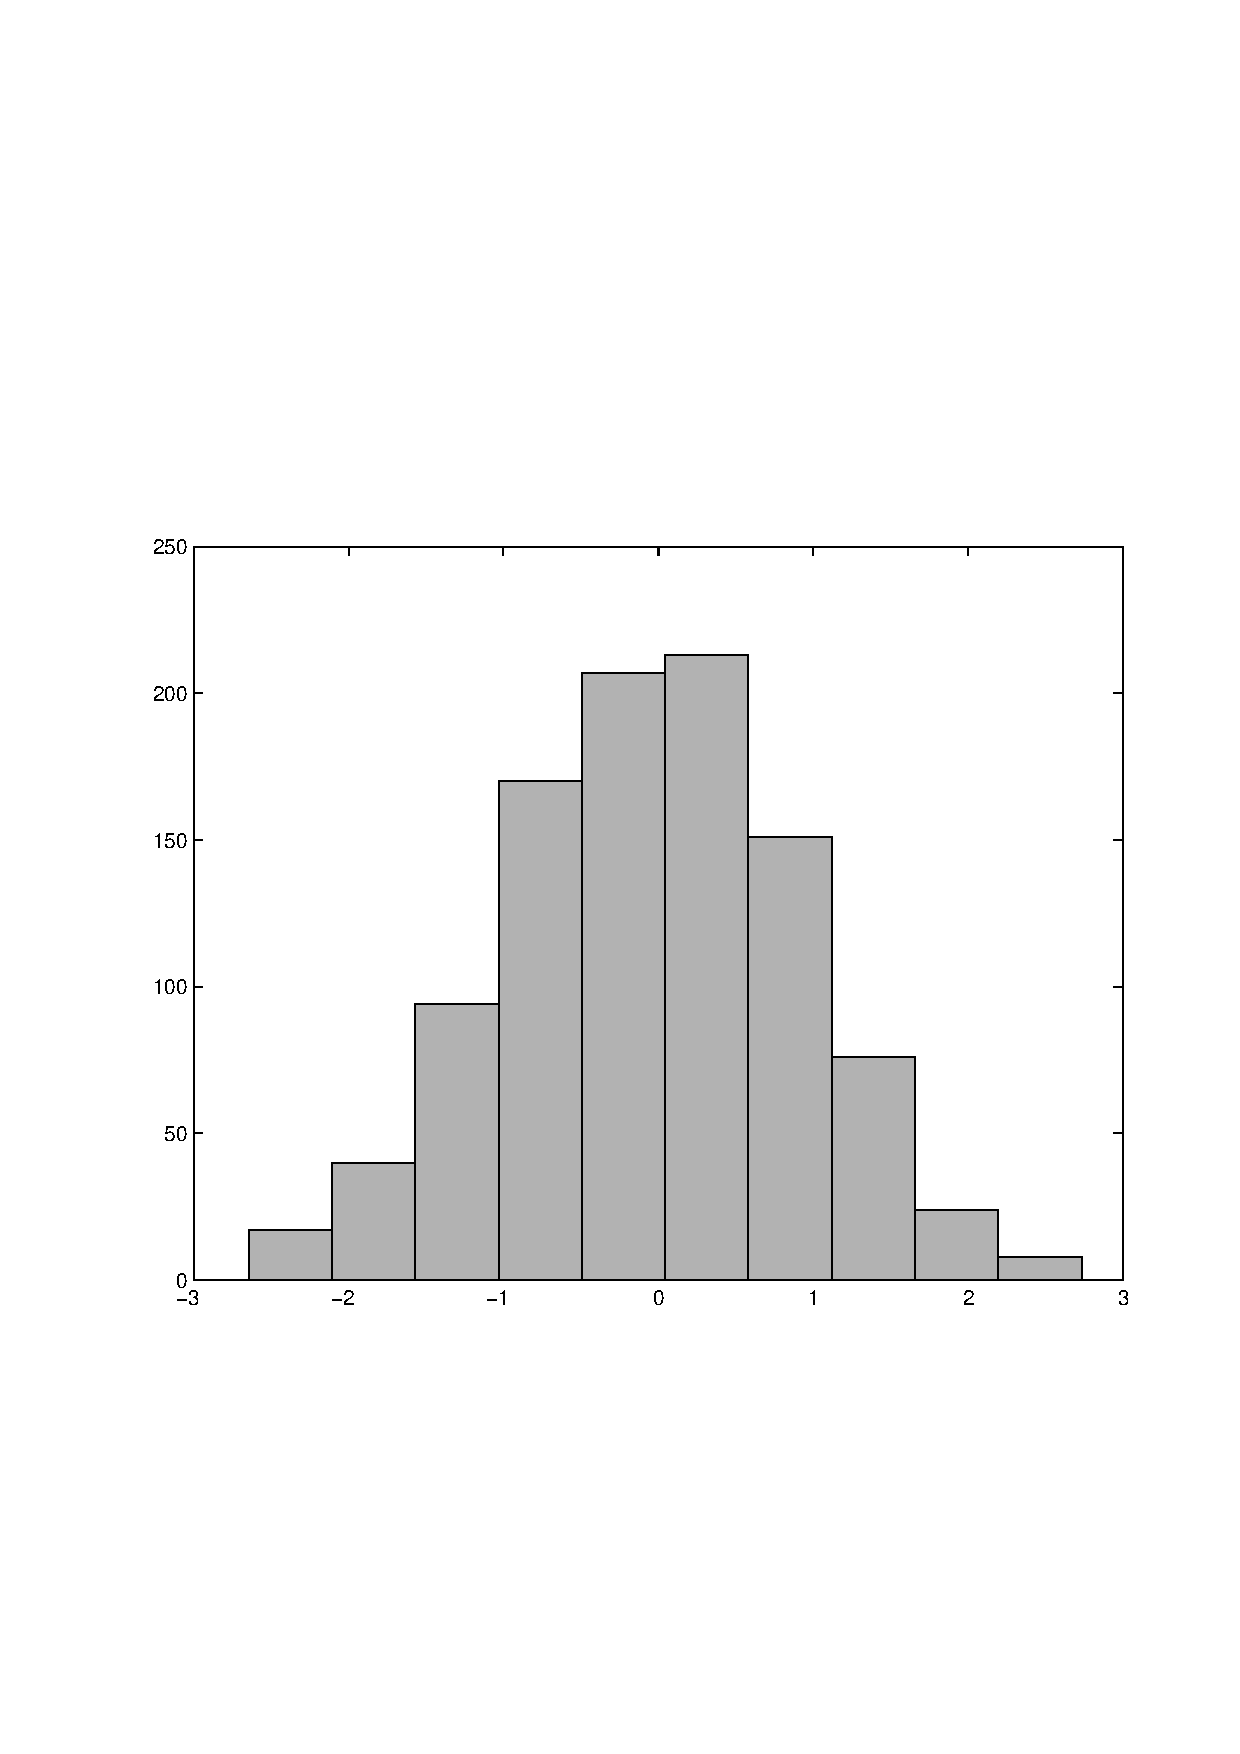
\includegraphics[width=0.3\textwidth]{fig}
	\caption{Histogram of 1000 normally distributed random
numbers.}
	\label{figlabel}
\end{figure}

\begin{figure}[H]
	\centering
	
\includegraphics[width=0.3\textwidth]{calvin}
	\caption{Another Figure with a png extension}
	\label{calvin}
\end{figure}



Note that the {\tt caption} command gives the figure a number that can be referred to later as Figure \ref{figlabel} and \ref{calvin}.

The file {\tt fig.pdf} was created in matlab with the commands:
\begin{verbatim}
     >> r = randn(1000,1);
     >> hist(r)             
     >> colormap([.7 .7 .7])    % to change the color and make it print better
     >> print fig.pdf
\end{verbatim}


\subsection{Tables}
Tables use below format. Note c refers to the columns, there are 3 columns in the first and second table, while the third table has 4 columns. Center means center the table in the page.  Following begin tabular, rows start, there are 3 rows here in~\ref{tab-1}, and each cell in a row is seperated by a \& and the row ends by using double backslash to move to next line.

\begin{table}[!h]
\begin{center}
\begin{tabular}{c c c}
 cell1 & cell2 & cell3 \\
 cell4 & cell5 & cell6 \\  
 cell7 & cell8 & cell9
\end{tabular}
\caption{Table-1 without border}
\label{tab-1}
\end{center}
\end{table}

Another table. A $|$ seperating the c's in the second Table~\ref{tab-2}, essentially draws a border. A hline draws a horizontal line.

\begin{table}[!h]
\begin{center}
\begin{tabular}{|c|c|c|}
 \hline
 cell1 & cell2 & cell3 \\
 hello & world & ! \\
 cell7 & cell8 & cell9 \\
 \hline
\end{tabular}
\caption{Table-2 with border}
\label{tab-2}
\end{center}
\end{table}

A more complex table with double lines in some places. Here, we applied the float placement specifier $\!h$ to place the table "here", encouraging LaTeX to locate it below the line of text. The [0.5ex] at the end of the headings row is used to add extra vertical spacing between the heading and the first row of the table. Similarly at the end.

\begin{table}[!h]
\begin{center}
\begin{tabular}{||c c c c||} 
 \hline
 Col1 & Col2 & Col2 & Col3 \\ [0.5ex] 
 \hline\hline
 1 & 6 & 87837 & 787 \\ 
 \hline
 2 & 7 & 78 & 5415 \\
 \hline
 3 & 545 & 778 & 7507 \\
 \hline
 4 & 545 & 18744 & 7560 \\
 \hline
 5 & 88 & 788 & 6344 \\ [1ex] 
 \hline
\end{tabular}
\caption{\label{demo-table}Your caption.}
\end{center}
\end{table}



\section{Bibliography and citations}
See a \LaTeX~ manual such as \cite{go-mi-sa:latex} for complete information on the use of a bibliography and citations. The main idea is the use of a bibliographic database such as the one in {\tt samplebib.bib}, which lists a large set of papers and books, each with a distinct label.  Then the  {\tt cite} command references one of the entries in the database by its label.  Hence, the citation is included in the paper; the corresponding reference is automatically included in the bibliography of the paper.  To do this, you must:
\begin{enumerate}
\item First run {\tt pdflatex sample}
\item Then run {\tt bibtex sample}
\item Then run {\tt pdflatex sample}
\item Then run {\tt pdflatex sample}
\end{enumerate}

The first run of \LaTeX~ creates a file {\tt sample.aux}
that contains information on the literature references.
Running bibtex then creates another file {\tt sample.bbl}, which is read into
the next \LaTeX~ run producing the list of literature references.  
Running \LaTeX~ twice more is needed to read in the citations with proper numbering. 

\bibliographystyle{plain}   % tells how to format bibliographic entries
\bibliography{sample}    % tells that the database is in sample.bib
\end{document} % This is the end of the document
